\subsection{Протокол Нидхема~---~Шрёдера}\index{протокол!Нидхема~---~Шрёдера|(}\label{section-protocols-needham-schroeder}
\selectlanguage{russian}

Протокол Нидхема~---~Шрёдера (\langen{Roger Needham, Michael Shroeder}, 1979,~\cite{Needham:Schroeder:1978}) похож на модифицированный протокол Wide-Mouth Frog, но отличается тем, что доверенный центр (Трент) во время работы основной части протокола не общается со вторым абонентом. Первый абонент получает от доверенного центра специальный пакет, который он без всякой модификации отправляет второму абоненту.

\begin{figure}
    \centering
    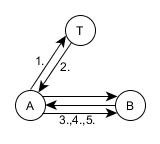
\includegraphics[width=0.5\textwidth]{pic/key_distribution-needham-schroeder}
    \caption{Схема взаимодействия абонентов и доверенного центра в протоколе Нидхема~---~Шрёдера\label{fig:key_distribution-needham-schroeder}}
\end{figure}

\begin{samepage}\begin{itemize}
	\item[(1)] $ Alice	\to \{ A, B, R_A \}						\to Trent $
	\item[(2)] $ Trent	\to \{ E_A \left( R_A, B, K, E_B \left( K, A \right) \right) \}	\to Alice $
	\item[(3)] $ Alice	\to \{ E_B \left( K, A \right) \}				\to Bob $
	\item[(4)] $ Bob	\to \{ E_K \left( R_B \right) \}				\to Alice $
	\item[(5)] $ Alice	\to \{ E_K \left( R_B - 1 \right) \}				\to Bob $
\end{itemize}\end{samepage}

Протокол удобен с точки зрения сетевого взаимодействия участников (рис.~\ref{fig:key_distribution-needham-schroeder}). И общение с доверенным центром, и с конечным участником (Бобом) начинается только по инициативе первого участника (Алисы). При возникновении любых проблем передачи пакетов их видит именно то лицо, которое заинтересованно в получении ключей и доступов\footnote{Сравните с протоколом Yahalom, в котором при возникновении проблемы общения Трента и Алисы на третьем проходе Тренту потребовалось бы уведомить об этом Боба, а Бобу, в свою очередь, Алису.}. И если бы общение шло с использование протокола TCP/IP, потребовалось бы всего 2 сессии протокола TCP для выработки ключа. Причём последнюю сессию можно не закрывать, а использовать как сессию для дальнейшего взаимодействия уже с ключом $K$.

Протокол обеспечивает и двустороннюю аутентификацию сторон, и, казалось бы, защиту от атак с повторной передачей (\langen{replay attack}). Последнее делается с помощью введения уже известных по модифицированному протоколу Wide-Mouth Frog случайных меток $R_A$ и $R_B$. Действительно, без знания ключа злоумышленник не сможет выдать себя за Алису перед Бобом (так как не сможет расшифровать пакет с зашифрованной меткой $R_B$).

Однако протокол уязвим к атаке с известным сеансовым ключом. Если злоумышленник сумеет в какой-то момент времени получить ранее использованный сессионный ключ $K$, он сможет убедить Боба, что он является Алисой, и что это новый сессионный ключ. Для этого ему понадобится переданный ранее по открытому каналу пакет из пункта 3 протокола.

\begin{itemize}
	\item[(1)] $ Eva \to \{ A, B, R_A \} \to Trent $
	\item[(2)] $ Trent \to \{ E_A \left( R_A, B, K, E_B \left( K, A \right) \right) \}	\to Alice $
	\item[(3)] $ Alice \to \{ E_B \left( K, A \right) \} \to Bob $
	\item[(4)] $ Bob \to \{ E_K \left( R_B \right) \} \to Alice $
	\item[(5)] $ Alice \to \{ E_K \left( R_B - 1 \right) \} \to Bob $
	\item[{}]  $\dots$ по прошествии некоторого времени $\dots$
	\item[(6)] $ Eva~(Alice) \to \{ E_B \left( K, A \right) \} \to Bob $
	\item[(7)] $ Bob \to \{ E_K \left( R_B \right) \} \to Eva~(Alice) $
	\item[(8)] $ Eva (Alice) \to \{ E_K \left( R_B - 1 \right) \} \to Bob $
\end{itemize}

Относительно мелкий недостаток протокола состоит ещё и в том, что во втором пакете доверенный центр в зашифрованном виде передаёт то, что в третьем шаге пересылается по открытому каналу ($E_B \left( K, A \right)$).

Если в протокол добавить метки времени, тем самым ограничив время возможного использования сессионного ключа, а также исправить мелкий недостаток с двойным шифрованием, можно получить протокол, который лежит в основе распространённого средства аутентификации <<Kerberos>> для локальных сетей.

\index{протокол!Нидхема~---~Шрёдера|)}
